% ============================================================
% Chapter 8: Problem 7 — The Irrationality and Transcendence of Certain Numbers
% ============================================================

\chapter{The Irrationality and Transcendence of \texorpdfstring{$e^\pi$}{e^pi}}

\begin{solvedbox}
Hilbert's seventh problem asks whether $e^\pi$ is transcendental. It is. The Gelfond--Schneider theorem (1934) proves that $a^b$ is transcendental whenever $a$ is algebraic (not $0$ or $1$) and $b$ is an irrational algebraic number. Since $e^\pi = (-1)^{-i}$, this theorem implies directly that $e^\pi$ is transcendental.
\end{solvedbox}

\section{Historical Context}

\subsection{What Does It Mean for a Number to Be Irrational, Algebraic, or Transcendental?}

Before we can appreciate the depth of Hilbert's question, we need to understand a hierarchy of ``complexity'' that mathematicians use to classify real (and complex) numbers. This hierarchy is one of the most beautiful ideas in all of number theory.

A real number is \textbf{rational} if it can be expressed as a fraction $p/q$ where $p$ and $q$ are integers with $q \neq 0$. The rational numbers---$\frac{1}{2}$, $-\frac{3}{4}$, $0 = \frac{0}{1}$, $7 = \frac{7}{1}$---are the numbers we encounter most readily in everyday life.

A real number that is \emph{not} rational is called \textbf{irrational}. The ancient Greeks discovered, to their astonishment, that $\sqrt{2}$ is irrational: there is no fraction equal to it. The proof is one of the most elegant arguments in mathematics, and we will review it in the exercises below.

But irrationality is only the first step on the ladder. An \textbf{algebraic number} is any real (or complex) number that is a root of a polynomial equation with integer coefficients:
\[
    a_n x^n + a_{n-1} x^{n-1} + \cdots + a_1 x + a_0 = 0, \qquad a_i \in \mathbb{Z}, \quad a_n \neq 0.
\]
Every rational number is algebraic (it is a root of $qx - p = 0$). But many irrational numbers are algebraic too: $\sqrt{2}$ is a root of $x^2 - 2 = 0$, and the golden ratio $\phi = \frac{1+\sqrt{5}}{2}$ is a root of $x^2 - x - 1 = 0$.

A real number that is \emph{not} algebraic---that is, a number that is not the root of \emph{any} polynomial with integer coefficients---is called \textbf{transcendental}. The name is poetic and apt: such numbers ``transcend'' the reach of algebraic equations.

Here is the hierarchy, from simplest to most exotic:

\[
    \underbrace{\mathbb{Q}}_{\text{rational}} \;\subset\; \underbrace{\text{algebraic numbers}}_{\text{roots of polynomials}} \;\subset\; \underbrace{\mathbb{R}}_{\text{real numbers}}
\]

The transcendental numbers are those real numbers that fall outside the algebraic numbers---the ``gaps'' in the algebraic landscape. For a long time, it was not even clear that transcendental numbers \emph{existed}. The proof that they do was one of the great achievements of 19th-century mathematics.

\begin{figure}[htbp]
\centering
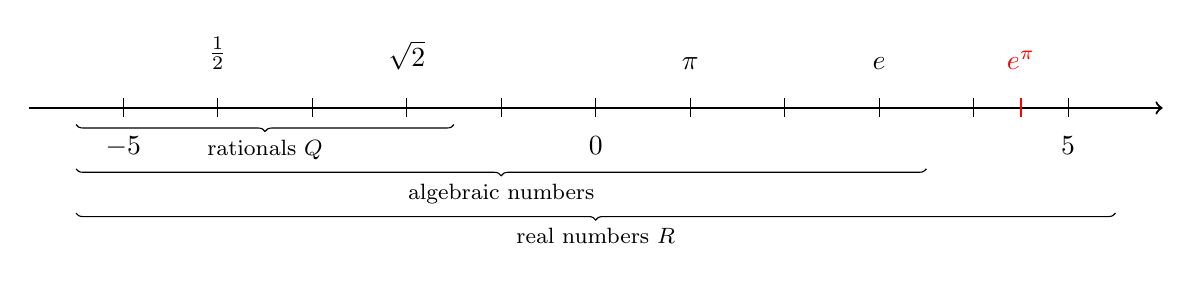
\begin{tikzpicture}[scale=1.2]
  \draw[thick,->] (-6,0) -- (6,0);
  \foreach \x in {-5,-4,-3,-2,-1,0,1,2,3,4,5} \draw (\x,0.1) -- (\x,-0.1);
  \node[below] at (-5,-0.2) {$-5$};
  \node[below] at (0,-0.2) {$0$};
  \node[below] at (5,-0.2) {$5$};
  \draw[decorate,decoration={brace,mirror,raise=6pt}] (-5.5,0) -- (-1.5,0)
    node[midway,below=8pt] {\footnotesize rationals $\mathbb{Q}$};
  \draw[decorate,decoration={brace,mirror,raise=22pt}] (-5.5,0) -- (3.5,0)
    node[midway,below=24pt] {\footnotesize algebraic numbers};
  \draw[decorate,decoration={brace,mirror,raise=38pt}] (-5.5,0) -- (5.5,0)
    node[midway,below=40pt] {\footnotesize real numbers $\mathbb{R}$};
  \node[above] at (-4,0.3) {$\frac{1}{2}$};
  \node[above] at (-2,0.3) {$\sqrt{2}$};
  \node[above] at (1,0.3) {$\pi$};
  \node[above] at (3,0.3) {$e$};
  \node[above,red] at (4.5,0.3) {$e^\pi$};
  \draw[red,thick] (4.5,0.1) -- (4.5,-0.1);
\end{tikzpicture}
\caption{Hierarchy of numbers: rationals, algebraic numbers, and reals, with examples. $e^\pi$ (in red) lies in the transcendental region outside the algebraic numbers.}
\label{fig:number-hierarchy}
\end{figure}

\subsection{The First Examples}

The first number proven to be transcendental was $e$ (Euler's number, approximately $2.71828\ldots$). In 1873, Charles Hermite proved that $e$ is transcendental. His proof was a tour de force of analysis, exploiting the rapidly converging series
\[
    e = \sum_{n=0}^{\infty} \frac{1}{n!}
\]
and the remarkable fact that this series converges so quickly that it ``outruns'' any polynomial approximation.

Nine years later, in 1882, Ferdinand Lindemann extended Hermite's methods to prove the transcendence of $\pi$. This was a landmark achievement, and it settled one of the oldest open problems in mathematics: the impossibility of \emph{squaring the circle}---constructing, with compass and straightedge alone, a square whose area equals that of a given circle. Since compass-and-straightedge constructions can only produce algebraic numbers, and $\pi$ is transcendental, the task is impossible.

\subsection{Lindemann's Proof That \texorpdfstring{$\pi$}{pi} Is Transcendental}

Lindemann's argument is beautiful in its broad outlines. We sketch the key idea.

Suppose, for contradiction, that $\pi$ is algebraic. Then $i\pi$ is also algebraic (since $i$ is algebraic: it is a root of $x^2 + 1 = 0$). By Euler's identity, $e^{i\pi} = -1$. So we would have an \emph{algebraic} exponent---$i\pi$---giving rise to an \emph{algebraic} value---$-1$---via the exponential function.

Lindemann proved a powerful general result that rules this out:

\begin{theorem}[Lindemann, 1882]
If $\alpha$ is a nonzero algebraic number, then $e^\alpha$ is transcendental.
\end{theorem}

The contrapositive is immediate: if $e^\alpha$ is algebraic and nonzero, then $\alpha$ must be transcendental. Taking $\alpha = i\pi$, we get $e^{i\pi} = -1$, which is algebraic and nonzero, so $i\pi$ must be transcendental---and therefore so is $\pi$.

The heart of Lindemann's proof lies in estimating certain ``auxiliary functions'' constructed from the exponential series. By choosing these functions carefully and using the assumption that $\alpha$ is algebraic, one derives a contradiction: an integer that is simultaneously very large and very small. This technique---assuming transcendence fails, building a clever approximation, and reaching a contradiction---became the prototype for virtually all subsequent work in transcendental number theory.

\section{The Problem}

\begin{problem_statement}
Is $e^\pi$ a transcendental number?
\end{problem_statement}

This may seem like a strange question. We already know that $e$ and $\pi$ are both transcendental. But the class of transcendental numbers is not ``closed'' under exponentiation: it is not at all obvious what happens when you raise one transcendental number to the power of another. Consider the following examples:

\begin{itemize}
    \item $e^e$ is not known to be transcendental (or even irrational!) as of this writing.
    \item $\pi^\pi$ is not known to be transcendental either.
    \item $\pi^{\sqrt{2}}$ was proven transcendental only in 2002 by Yu. V. Nesterenko.
\end{itemize}

So the question ``Is $e^\pi$ transcendental?'' is not trivial at all. It requires a fundamentally new idea.

There is one observation, however, that connects $e^\pi$ to a more tractable framework. Consider the quantity $(-1)^{-i}$. Using Euler's identity $e^{i\pi} = -1$, we can write:
\[
    (-1)^{-i} = \left(e^{i\pi}\right)^{-i} = e^{\pi}.
\]
So $e^\pi = (-1)^{-i}$. Now $-1$ is algebraic (it is a root of $x + 1 = 0$), and $-i$ is algebraic and irrational (it is a root of $x^2 + 1 = 0$, and it is clearly not rational). If we had a theorem saying ``$a^b$ is transcendental whenever $a$ is algebraic (not $0$ or $1$) and $b$ is irrational algebraic,'' we would be done.

This is exactly what the Gelfond--Schneider theorem says.

\section{Key Developments}

\subsection{The Gelfond--Schneider Theorem}

In 1934, independently and almost simultaneously, Alexander Gelfond and Theodor Schneider proved one of the crown jewels of 20th-century number theory:

\begin{theorem}[Gelfond--Schneider, 1934]
Let $a$ and $b$ be algebraic numbers with $a \neq 0, 1$ and $b$ irrational. Then $a^b$ is transcendental.
\end{theorem}

The power of this theorem is immense. Here are some of its immediate consequences:

\begin{itemize}
    \item $2^{\sqrt{2}}$ is transcendental. (Here $a = 2$, $b = \sqrt{2}$, and $\sqrt{2}$ is irrational.)
    \item $e^\pi$ is transcendental, via the identity $e^\pi = (-1)^{-i}$. Here $a = -1$ (algebraic, not $0$ or $1$), and $b = -i$ (algebraic and irrational).
    \item Any value of $\log 2$---that is, any complex number $\alpha$ such that $e^\alpha = 2$---is transcendental.
\end{itemize}

\subsection{Why \texorpdfstring{$e^\pi$}{e^pi} Is Transcendental: The Clever Trick}

Let us spell out the argument for $e^\pi$ in detail, since it is one of the most beautiful deductions in all of mathematics.

We begin with Euler's identity:
\[
    e^{i\pi} = -1.
\]
Raise both sides to the power $-i$:
\[
    \left(e^{i\pi}\right)^{-i} = (-1)^{-i}.
\]
The left side simplifies: $\left(e^{i\pi}\right)^{-i} = e^{(-i)(i\pi)} = e^{\pi}$.\linebreak[0] So:
\[
    e^\pi = (-1)^{-i}.
\]
Now apply the Gelfond--Schneider theorem with $a = -1$ and $b = -i$:
\begin{itemize}
    \item $a = -1$ is algebraic and $a \neq 0, 1$.
    \item $b = -i$ is algebraic (root of $x^2 + 1 = 0$) and irrational (not a ratio of integers).
\end{itemize}
Therefore $a^b = (-1)^{-i} = e^\pi$ is transcendental.

This is a remarkable chain of reasoning: we start with the geometry of the circle (Euler's identity connects $e$, $\pi$, and $i$), apply a deep theorem about algebraic exponents, and conclude something profound about a concrete, computable constant.

\subsection{The Proof Idea of Gelfond--Schneider}

The proof of the Gelfond--Schneider theorem is technically demanding, but its broad strategy can be described. It is a generalization and refinement of Hermite's and Lindemann's methods.

The key idea is to construct an \emph{auxiliary function}---a carefully designed analytic function that satisfies two contradictory properties simultaneously:

\begin{enumerate}
    \item On one hand, the function is ``too small'' to be nonzero at certain algebraic points (by an application of the pigeonhole principle or a version of Dirichlet's approximation theorem).
    \item On the other hand, the function cannot be exactly zero at those points, because doing so would force a polynomial relation with algebraic coefficients that cannot exist.
\end{enumerate}

This contradiction shows that the original assumption---that $a^b$ is algebraic---must be false.

The technical heart of the proof involves estimating the size of certain linear forms in logarithms:
\[
    \Lambda = \beta_1 \log \alpha_1 + \beta_2 \log \alpha_2 + \cdots + \beta_n \log \alpha_n,
\]
where the $\alpha_i$ and $\beta_i$ are algebraic numbers. Showing that such a linear form cannot be too close to zero (when it is nonzero) is the central problem of the field.

\subsection{Baker's Theorem: Linear Forms in Logarithms}

The Gelfond--Schneider theorem was extended dramatically by Alan Baker in 1966. Baker proved the following far-reaching generalization:

\begin{theorem}[Baker, 1966]
If $\alpha_1, \ldots, \alpha_n$ are nonzero algebraic numbers and $\beta_1, \ldots, \beta_n$ are algebraic with $1, \beta_1, \ldots, \beta_n$ linearly independent over $\mathbb{Q}$, then\linebreak
\[
    \beta_1 \log \alpha_1 + \beta_2 \log \alpha_2 + \cdots + \beta_n \log \alpha_n \neq 0.
\]
\end{theorem}

In other words, nontrivial linear combinations of logarithms of algebraic numbers with algebraic coefficients are never zero---and Baker's work also gives effective lower bounds on how far such combinations can be from zero. This quantitative aspect is crucial for applications: it allows one to prove \emph{effectively} that certain numbers are transcendental, and even to bound their algebraic approximations.

Baker's theorem implies the Gelfond--Schneider theorem as a special case, and it has vast applications in Diophantine equations, the theory of transcendental numbers, and even in computational number theory.

The Gelfond--Schneider theorem is sometimes called one of the four fundamental theorems of transcendental number theory, alongside the Lindemann--Weierstrass theorem, Baker's theorem, and the six exponentials theorem. Together, these results give us a powerful toolkit for proving that specific numbers are transcendental.

\section{Current Status}

\begin{solvedbox}
Hilbert's seventh problem is \textbf{solved}. The Gelfond--Schneider theorem (1934) proves that $e^\pi$ is transcendental. The broader question of which values of $a^b$ are transcendental is largely settled by the Gelfond--Schneider theorem and Baker's theorem, though many specific questions remain open.
\end{solvedbox}

Despite these triumphs, transcendental number theory remains a field of deep open problems. Among the most famous:

\begin{itemize}
    \item \textbf{Is $\pi + e$ transcendental?} We know that both $\pi$ and $e$ are transcendental, but we do not know whether their sum is. It is conjectured to be, but no proof is known.
    \item \textbf{Is $\pi \cdot e$ transcendental?} Again, unknown. It is even unknown whether $\pi^e$ is irrational.
    \item \textbf{Is $2^e$ transcendental?} This is not known. Note that $2$ is algebraic and $e$ is \emph{not} algebraic, so the Gelfond--Schneider theorem does not apply.
    \item \textbf{Schanuel's conjecture.} This sweeping conjecture, if true, would resolve a vast number of open questions about transcendence. It states that if $\alpha_1, \ldots, \alpha_n$ are complex numbers that are linearly independent over $\mathbb{Q}$, then the transcendence degree of the field $\mathbb{Q}(\alpha_1, \ldots, \alpha_n, e^{\alpha_1}, \ldots, e^{\alpha_n})$ over $\mathbb{Q}$ is at least $n$. Nearly all major open problems in transcendental number theory are consequences of Schanuel's conjecture.
\end{itemize}

\section*{Common Questions}

\begin{description}[font=\bfseries, leftmargin=2em, style=nextline]

\item[Q: If $e$ and $\pi$ are both transcendental, why isn't $e \times \pi$ obviously transcendental?]\hfill\\
Transcendental numbers are not closed under addition, multiplication, or exponentiation. Knowing that each of two numbers is transcendental tells you nothing about their sum or product. For example, $\pi$ and $1-\pi$ are both transcendental (if $1-\pi$ were algebraic, then $\pi = 1 - (1-\pi)$ would be algebraic), yet $\pi + (1-\pi) = 1$ is rational. Similarly, $e$ and $\ln 2$ are both transcendental, yet $e^{\ln 2} = 2$ is algebraic. So the transcendence of $e$ and $\pi$ individually gives no information about $e \times \pi$, $e + \pi$, or $\pi^e$.

\item[Q: How does $e^\pi = (-1)^{-i}$ help? Isn't $(-1)^{-i}$ just as mysterious?]\hfill\\
The trick is that $(-1)^{-i}$ rewrites the problem in a form where the Gelfond--Schneider theorem applies. That theorem requires an algebraic base (not $0$ or $1$) and an irrational algebraic exponent. $-1$ is algebraic (it is a root of $x+1=0$), and $-i$ is algebraic (a root of $x^2+1=0$) and irrational. The theorem then guarantees that $(-1)^{-i}$---and therefore $e^\pi$---is transcendental. So the identity transforms an intractable-looking problem into one that fits neatly into a known framework.

\item[Q: What's the difference between irrational and transcendental?]\hfill\\
Every real number fits into a four-tier hierarchy. \textbf{Rational} numbers are fractions $p/q$ ($\frac{1}{2}, 7$). \textbf{Algebraic} numbers are roots of polynomials with integer coefficients ($\sqrt{2}, \phi$). All rationals are algebraic, but not all algebraic numbers are rational. \textbf{Irrational} simply means ``not rational,'' so it includes both algebraic irrationals ($\sqrt{2}$) and transcendental numbers ($\pi$). \textbf{Transcendental} means ``not algebraic''---the number is not a root of any polynomial with integer coefficients. So $\sqrt{2}$ is irrational but not transcendental; $\pi$ is both irrational and transcendental. The step from irrational to transcendental is enormous: proving a number is transcendental is vastly harder than proving it is irrational.

\item[Q: Are there any known numbers that we haven't proven are either rational or irrational?]\hfill\\
Yes, many. The most famous examples are $e + \pi$, $e \times \pi$, and $\pi^e$. Nobody has proved whether any of these is rational or irrational (let alone transcendental). It is conjectured that all three are transcendental, but no proof exists. Even simpler-sounding numbers like $\gamma$ (the Euler--Mascheroni constant) and $\zeta(5)$ (Apéry's constant is known only for $\zeta(3)$) are not known to be rational or irrational. This shows how primitive our understanding remains despite the power of transcendental number theory.

\item[Q: Why was Hilbert's seventh problem considered important enough for his list?]\hfill\\
Hilbert's list aimed at foundational questions whose resolution would advance mathematics broadly. The transcendence of $e^\pi$ was a test case for a much deeper issue: understanding the relationship between algebraic numbers and exponentials. Solving it required the Gelfond--Schneider theorem, which gave a general criterion that settled the problem and opened up the entire field of transcendental number theory. The result also had concrete implications---for example, it immediately implies that $2^{\sqrt{2}}$ is transcendental, and it paved the way for Baker's theorem, which has applications in Diophantine equations and computational number theory.

\item[Q: Can the Gelfond--Schneider theorem tell us whether $\pi^e$ is transcendental?]\hfill\\
No. The theorem requires that the \emph{exponent} be an algebraic irrational number. In $\pi^e$, the exponent $e$ is transcendental, not algebraic, so the theorem does not apply. In fact, $\pi^e$ is not even known to be irrational. The case where both base and exponent are transcendental is wide open in general. This asymmetry underscores why $e^\pi$ was tractable (via $(-1)^{-i}$) while $\pi^e$ remains stubbornly mysterious.

\item[Q: What does ``effectively computable'' mean in the context of Baker's theorem?]\hfill\\
Baker's theorem provides explicit lower bounds on how close a linear combination of logarithms of algebraic numbers can be to zero. ``Effectively computable'' means that given specific algebraic numbers, you can actually calculate a concrete number $C > 0$ such that the linear form must be larger than $C$ (unless it is identically zero). This is crucial for applications: it means you can algorithmically bound how large a solution to a Diophantine equation can be, which often reduces solving the equation to checking finitely many cases. Without effective bounds, you would know a solution cannot be too close to zero, but you wouldn't know how close is ``too close.''

\end{description}

\section*{Exercises}

\begin{enumerate}
    \item \textbf{Proving $\sqrt{2}$ is irrational (review).}
    \begin{enumerate}
        \item Suppose $\sqrt{2} = p/q$ where $p$ and $q$ are positive integers with no common factors. Show that $p^2 = 2q^2$ and deduce that $p$ is even.
        \item Write $p = 2k$ and show that $q$ must also be even, contradicting the assumption that $p/q$ is in lowest terms.
        \item Conclude that $\sqrt{2}$ is irrational.
        \item \textbf{Generalize:} adapt this argument to prove that $\sqrt{n}$ is irrational for any positive integer $n$ that is not a perfect square. (Hint: if $n$ is not a perfect square, consider the prime factorization of $n$.)
    \end{enumerate}

    \item \textbf{Proving $e$ is irrational.}
    \begin{enumerate}
        \item Suppose $e = p/q$ where $p$ and $q$ are positive integers. Using the series $e = \sum_{n=0}^{\infty} \frac{1}{n!}$, multiply both sides by $q!$ and consider the remainder:
        \[
            q! \, e = q! \sum_{n=0}^{\infty} \frac{1}{n!} = \underbrace{\sum_{n=0}^{q} \frac{q!}{n!}}_{\text{integer}} + \underbrace{\sum_{n=q+1}^{\infty} \frac{q!}{n!}}_{\text{remainder}}.
        \]
        \item Show that the remainder satisfies $0 < \sum_{n=q+1}^{\infty} \frac{q!}{n!} < 1$.
        \item Deduce that $q! \, e$ is not an integer, contradicting the assumption that $e = p/q$.
    \end{enumerate}

    \item \textbf{Algebraic numbers: examples and non-examples.}
    \begin{enumerate}
        \item Show that $\sqrt{2} + \sqrt{3}$ is algebraic by finding a polynomial with integer coefficients that has it as a root.
        \item Is $\sqrt{2} \cdot \sqrt{3} = \sqrt{6}$ algebraic? Find its minimal polynomial.
        \item Show that the set of algebraic numbers is a field (closed under addition, subtraction, multiplication, and division by nonzero elements). This is a nontrivial fact---can you explain why it is true? (Hint: the set of roots of a product of two polynomials with integer coefficients is finite and closed under the relevant operations.)
    \end{enumerate}

    \item \textbf{The Gelfond--Schneider theorem in action.} Apply the Gelfond--Schneider theorem to determine whether each of the following numbers is transcendental:
    \begin{enumerate}
        \item $3^{\sqrt{5}}$
        \item $(-1)^{\sqrt{2}}$ (Hint: write $(-1)^{\sqrt{2}} = e^{\sqrt{2} \cdot \pi i}$ and think carefully.)
        \item $2^{i}$
        \item $i^i$ (Hint: $i^i = e^{i \cdot \log i} = e^{i \cdot (i\pi/2)} = e^{-\pi/2}$.)
    \end{enumerate}

    \item \textbf{Historical reflection.} The ancient Greeks knew that $\sqrt{2}$ is irrational, yet it took over two thousand years to prove that $\pi$ is transcendental. Why was the transcendence of $\pi$ so much harder? Discuss the gap between proving irrationality and proving transcendence.

    \item $\star$ \textbf{Schanuel's conjecture.} Schanuel's conjecture (stated in the chapter) would imply, among other things, that $\pi + e$, $\pi \cdot e$, and $\pi^e$ are all transcendental. Verify this for $\pi + e$: assuming Schanuel's conjecture, explain why $\pi + e$ must be transcendental. (Hint: apply Schanuel's conjecture with $n = 2$, $\alpha_1 = \pi i$, $\alpha_2 = 1$. Note that $e^{\pi i} = -1$ and $e^1 = e$.)
\end{enumerate}
